\section{Auswertung}
\label{sec:Auswertung}

In dem zur Messung verwendeten Programm kann zwischen den verschiedenen Einstellmöglichkeiten AM, HF und AM + HF gewählt werden.
Dabei steht AM für Amplitude und HF für die Einhüllende der Amplitude. Wird die Einstellung AM + HF gewählt, so wird sowohl die Amplitude in rot, 
als auch die Einhüllende in blau eingezeichnet. Diese Einstellung wurde in den folgenden Grafiken gewählt. \newline
Im folgenden werden die grundlegenden Eigenschaften des Ultraschalles, die in dem Versuch untersucht wurden, ausgewertet.
Zunächst wurden die verwendeten Acrylplatten mit einer Schieblehre abgemessen, um die Werte später mit denen des Ultraschallgerätes vergleichen zu können. 
Die gemessenen Werte der Plattendicke lauten wie folgt,
\begin{align*}
  P_1 &= \SI{10}{\mm}, \\
  P_2 &= \SI{6}{\mm}.
\end{align*}
Die in \autoref{fig:reflexe} aufgenommene Grafik zeigt die vier Reflexe, die mit dem Puls-Echo-Verfahren aufgenommen wurden. Die Amplituden und Laufzeiten, 
die sich aus diesen Reflexen ergeben sind in \autoref{tab:refl} eingetragen. Die Mittelwerte der Laufzeiten und der Amplituden sind ebenfalls in der Tabelle eingetragen.

\begin{figure}[H]
  \centering
  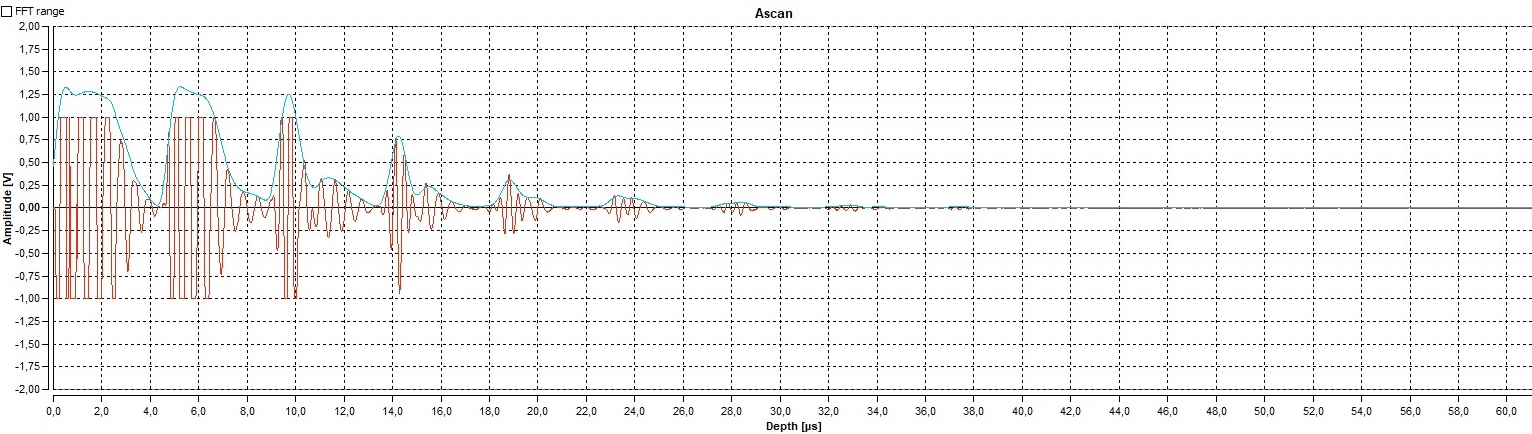
\includegraphics[width = \textwidth]{data/Geräteeinstellungen/reflexe.png}
  \caption{Aufgenommene Grafik zu den vier Reflexen.}
  \label{fig:reflexe}
\end{figure}

\begin{table}
  \centering
  \caption{Auswertung der aufgenommenen Grafik zu den vier Reflexen.}
  \label{tab:refl}
  \begin{tabular}{c c c}
    \toprule
    Reflex $R_i$ & Laufzeit / $\si{\micro\second}$ & Amplitude / $\si{\volt}$ \\
    \midrule
    $R_1$ & 4,0 & 1,30 \\
    $R_2$ & 4,9 & 1,30 \\
    $R_3$ & 4,8 & 1,25 \\
    $R_4$ & 3,2 & 0,80 \\
    $\overline R$ & $4.2 \pm 0.7$ & $1.16 \pm 0.21$ \\
    \bottomrule
  \end{tabular}
\end{table}
Die theoretische Periodenlänge ergibt sich über die eingestellte Frequenz von $\SI{2}{\mega\hertz}$ zu 
\begin{align*}
  T = \frac{1}{\SI{2}{\mega\hertz}} = \SI{0,5}{\micro\second}.
\end{align*}
Die Schwingungsperioden sind aus \autoref{fig:schwingungen} ausgewertet worden und ihre Ergebnisse sind aus \autoref{tab:perids} zusammen mit dem Mittelwert der Schwingungen $\overline{S_i}$ abzulesen.

\begin{figure}[H]
  \centering
  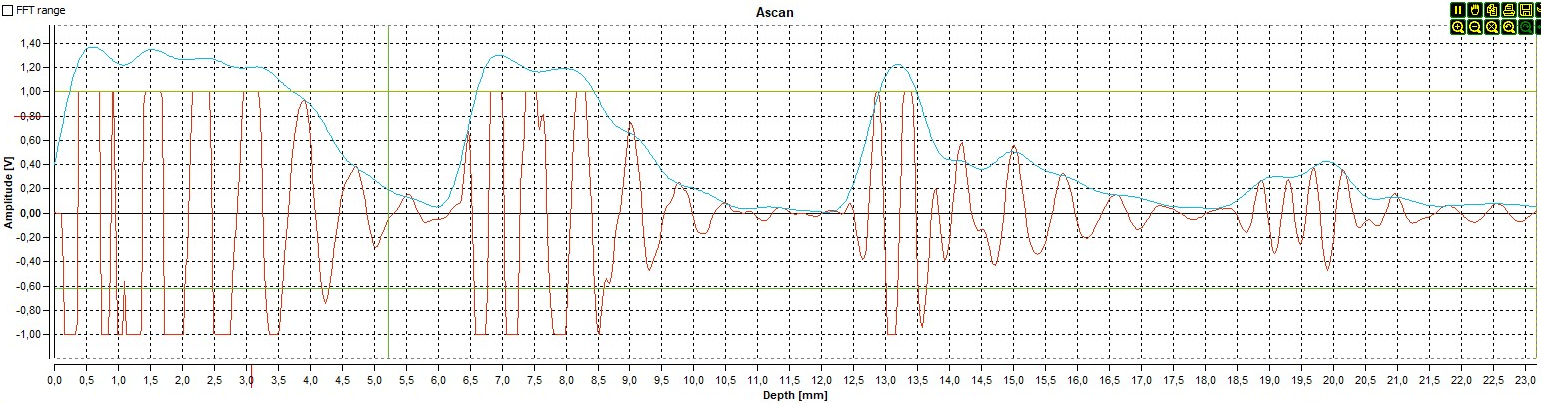
\includegraphics[width = \textwidth]{data/Geräteeinstellungen/schwingung.png}
  \caption{Aufgenommene Grafik zur Auswertung der Schwingungsperioden.}
  \label{fig:schwingungen}
\end{figure}

\begin{table}
  \centering
  \caption{Auswertung der aufgenommenen Grafik zu den Schwingungsperioden.}
  \label{tab:perids}
  \begin{tabular}{c c}
    \toprule
    Schwingung $S_i$ & Periodenlänge / $\si{\micro\second}$  \\
    \midrule
    $S_1$ & 0,50 \\
    $S_2$ & 0,54 \\
    $S_3$ & 0,58 \\
    $S_4$ & 0,54 \\
    $S_5$ & 0,57 \\
    $\overline{S_i}$ & $0.546 \pm 0.028$ \\
    \bottomrule
  \end{tabular}
\end{table}

Mithilfe des Ultraschallgerätes wird die Dicke der Acrylplatte bestimmt. Die dazu angefertigte Grafik ist in \autoref{fig:acrylplatte} dargestellt.
Der erste Peak ist die reflektierte Intensität an der Wasseroberfläche der Acrylplatte und deshalb für die Auswertung der Plattendicke überflüssig. Die Länge des zweiten Peaks beschreibt die Dicke des Acryls.
Es wird eine Tiefe von $D = \SI{6}{\milli\meter}$ bestimmt.

\begin{figure}[H]
  \centering
  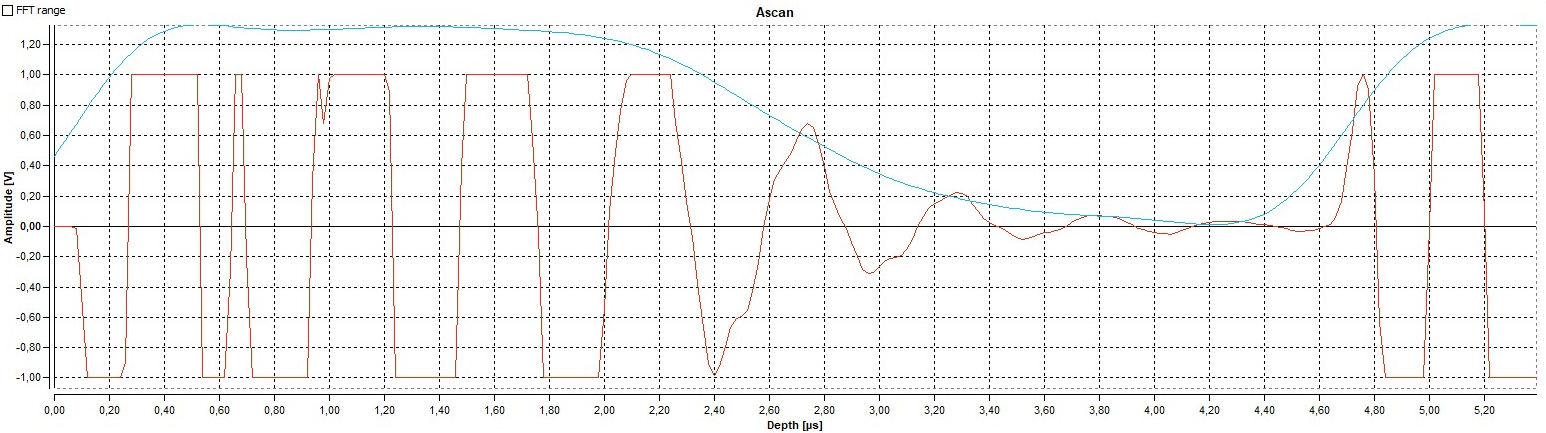
\includegraphics[width = \textwidth]{data/Geräteeinstellungen/tiefe.png}
  \caption{Aufgenommene Grafik zur Auswertung der Dicke der Acrylplatte.}
  \label{fig:acrylplatte}
\end{figure}

\subsection{Auswertung der Schallgeschwindigkeit mithilfe des Impuls-Echo-Verfahrens}
\label{subsec:schallImpEcho}

Mithilfe eines Amplituden-Scans soll nun die Laufzeit des Echos in einem Acrylzylinder ausgewertet werden. Die Laufzeiten sind in \autoref{tab:tiefeZyls} mit einem Mittelwert eingetragen.
Es wurden dabei die vier verschiedenen Zylinder ausgemessen, die in dem Versuch zur Verfügung standen. Der Grund, weshalb keine Messwerte genommen wurde als die Zylinder aufeinandergestapelt waren, 
wird in \autoref{sec:Diskussion} erklärt. %Die Kombinationen sind in der Zylinderkennzeichnung markiert.
Die mit der Schieblehre ausgemessenen Längen und Durchmesser sind ebenfalls eingetragen, um sie miteinander vergleichen zu können.
Außerdem sind die berechneten Schallgeschwindigkeiten $\nu$ in \autoref{tab:tiefeZyls} eingetragen.
Die Schallgeschwindigkeiten berechnen sich aus
\begin{align}
  s = \frac 12 \nu t \iff \nu = \frac{2s}{t}.
\end{align}

\begin{table}
  \centering
  \caption{Auswertung der aufgenommenen Grafik zu den Schwingungsperioden.}
  \label{tab:tiefeZyls}
  \begin{tabular}{c c c c c}
    \toprule
    Zylinder $Z_i$ & Länge / $\si{\milli\meter}$  &  Laufzeiten / $\si{\micro\second}$ & Durchmesser / $\si{\milli\meter}$ & $\nu_1$ / $\si{\meter\per\second\squared} $\\
    \midrule
    $Z_1$ & 40,4  & 18,32 & 40,0 & 2205,24\\
    $Z_2$ & 61,5  & 34,43 & 40,0 & 1786,23 \\
    $Z_3$ & 80,5  & 43,96 & 40,5 & 1831,21 \\
    $Z_4$ & 120,5 & 79,12 & 40,0 & 1523,01 \\
    % $Z_14$  & 160, & 32   \\
    % $Z_42$  &  &  88  \\
    % $Z_43$  &  & 74   \\
    % $Z_123$ &  & 68   \\    
    \bottomrule
  \end{tabular}
\end{table}

Der Mittelwert der Schallgeschwindigkeiten ergibt sich somit zu
\begin{align*}
  \overline \nu_1 = \SI{1.84 \pm 0,24 e3}{\meter\per\second\squared}.
\end{align*}

\subsection{Auswertung der Schallgeschwindigkeit mithilfe des Durchschallungs-Verfahrens}
\label{subsec:schallDurch}

Die Schallgeschwindigkeiten sollen nun nocheinmal mithilfe des Durchschallungsverfahren bestimmt werden.
Die mithilfe des Amplituden-Scans bestimmten Laufzeiten und zugehörigen Schallgeschwindigkeiten der jeweiligen Zylinder sind in \autoref{tab:durchZyl} eingetragen.

\begin{table}
  \centering
  \caption{Auswertung der aufgenommenen Laufzeiten.}
  \label{tab:durchZyl}
  \begin{tabular}{c c c c c}
    \toprule
    Zylinder $Z_i$ &  Laufzeiten / $\si{\micro\second}$ & $\nu_2$ / $\si{\meter\per\second\squared} $\\
    \midrule
    $Z_1$ & 30,04 & 2689.75 \\
    $Z_2$ & 43,96 & 2797.99 \\
    $Z_3$ & 59,34 & 2713.18 \\
    $Z_4$ & 88,28 & 2729.95 \\
    \bottomrule
  \end{tabular}
\end{table}

Ein Mittelwert für die Schallgeschwindigkeit beim Durchschallungs-Verfahren erfolgt somit zu
\begin{align*}
  \overline \nu_2 = \SI{2,73 \pm 0,04 e3}{\meter\per\second\squared}.
\end{align*}

\subsection{Auswertung der Dämpfung mithilfe der Impuls-Echo-Methode}
\label{subsec:daempfung}

Es wird nun mithilfe der Impuls-Echo-Methode und einem A-Scan die Dämpfung des Acrylzylinders ausgewertet.
Es werden dabei die Amplituden der reflektierten Impulse gemessen und ausgewertet.
Weil die Amplituden mit Verstärkungen versehen sind, müssen sie erst korrigiert werden. Dazu wird die unverstärkte Amplitude $V_1$
mit dem folgenden Faktor multipliziert, um die tatsächliche Amplitude $V_2$ zu erhalten,
\begin{align*}
  Q \text dB &= 10\log\left(\frac{V_2}{V_1}\right) \text dB,\\
  \iff V_2 &= V_1\exp{\left(\frac{Q}{10}\right) }.
\end{align*}
Die Daten sind in \autoref{tab:amplis} eingetragen und in \autoref{fig:plot} grafisch ausgewertet.

\begin{table}
  \centering
  \caption{Auswertung der aufgenommenen Laufzeiten.}
  \label{tab:amplis}
  \begin{tabular}{c c c c c}
    \toprule
    Zylinder $Z_i$ &  Amplitude / $\si{\volt}$ \\
    \midrule
    $Z_1$ & 0,78 \\
    $Z_2$ & 2.11 \\
    $Z_3$ & 21.63 \\
    $Z_4$ & 3.72 \\
    \bottomrule
  \end{tabular}
\end{table}

Mithilfe der Python-Erweiterungen numpy \cite{numpy}, matplotlib \cite{matplotlib} und scipy \cite{scipy} wird eine lineare Ausgleichsgerade
der Form
\begin{align*}
  y = m\cdot x + b,
\end{align*}
in die Grafik \ref{fig:plot} eingebaut. Die Parameter ergeben sich zu
\begin{align*}
  m = 0,0348 \pm 0.0072 \left[\si{\volt\per\meter}\right], \quad b = -0,4139 \pm 0,59 \left[\si{\volt}\right].
\end{align*}

\begin{figure}[H]
  \centering
  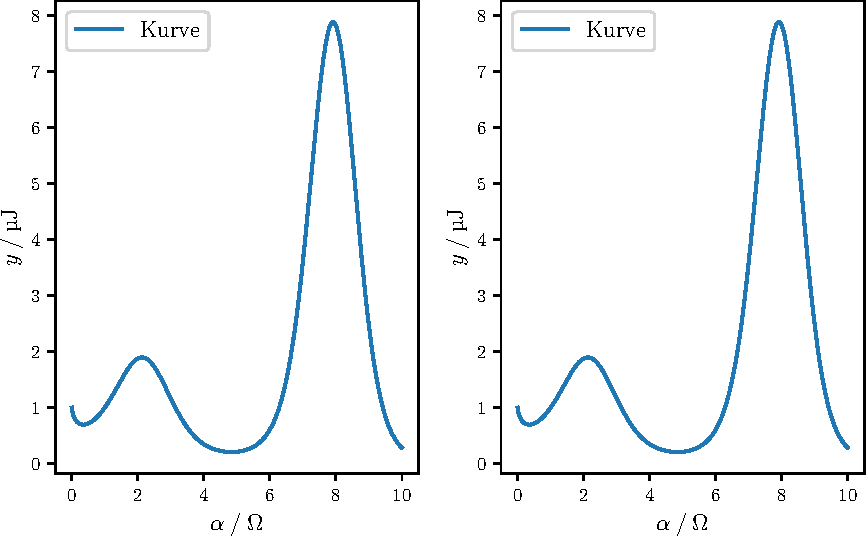
\includegraphics[width = \textwidth]{plot.pdf}
  \caption{Grafische Auswertung.}
  \label{fig:plot}
\end{figure}

\subsection{Biometrische Auswertung eines Augenmodells}
\label{subsec:auge}

Im folgenden werden die Abstände der Augapfelbestandteile eines Modellauges mithilfe von Ultraschall bestimmt. 
Dazu wird mit einem A-Scan und der Impuls-Echo Methode der in \autoref{fig:augePlot} dargestellte Verlauf erstellt.

\begin{figure}[H]
  \centering
  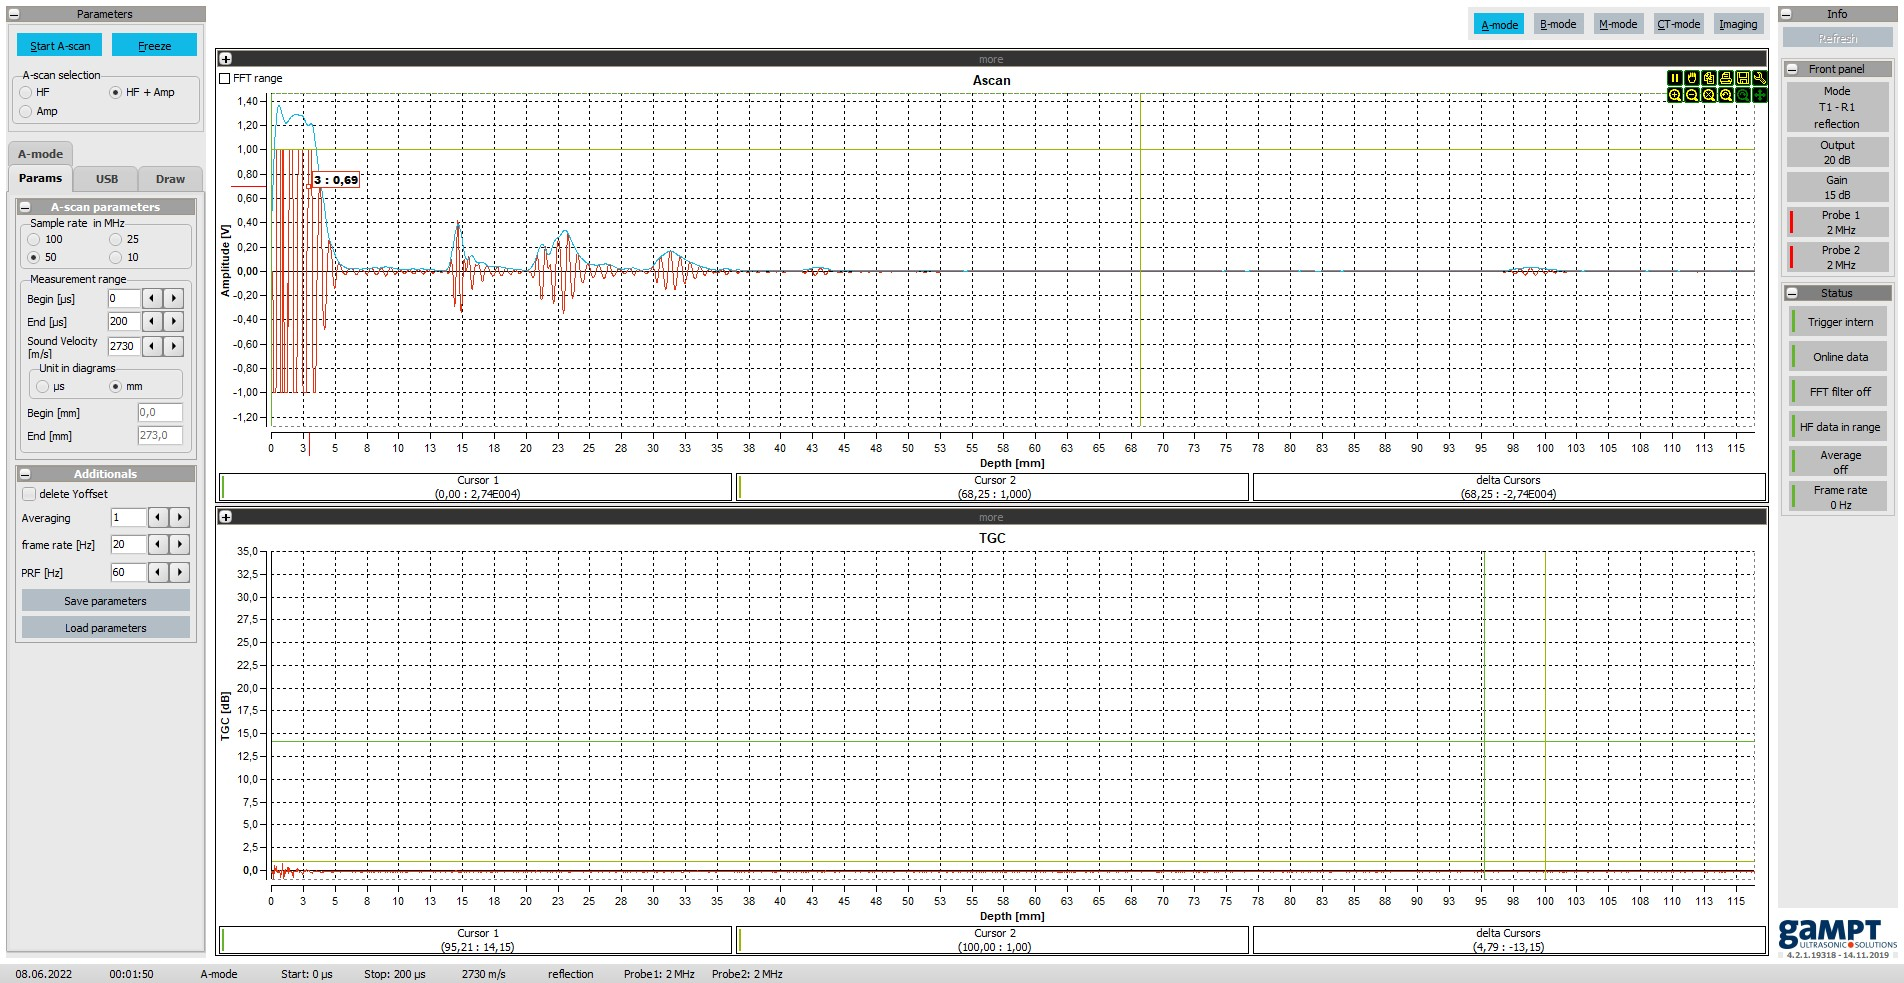
\includegraphics[width = \textwidth]{data/Auge.png}
  \caption{Grafische Darstellung der Messwerte eines Augapfelmodells.}
  \label{fig:augePlot}
\end{figure}

Die Peaks stellen die verschiedenen Bestandteile des Auges dar und lauten wie folgt,
\begin{align*}
  s_{\text{Iris}} &= \SI{14,9}{\mm}, \\
  s_{\text{Linse}} &= \SI{23,5}{\mm}, \\
  s_{\text{Retina}} &= \SI{43,7}{\mm}.
\end{align*}
Der dritte Peak ist die Relfexion der Linse, die wieder an der Ultraschallsonde des Gerätes detektiert wird.